\documentclass[12pt,a4paper]{article}
\usepackage[utf8]{inputenc}
\usepackage[english]{babel}

\usepackage{amsmath}
\usepackage{amsfonts}
\usepackage{amssymb}

\usepackage{graphicx}
\usepackage{lmodern}
\usepackage{tikz}
\usepackage{titlesec}
\usepackage{environ}
\usepackage{xcolor}
\usepackage{fancyhdr}
\usepackage[colorlinks = true, linkcolor = black]{hyperref}
\usepackage{xparse}
\usepackage{enumerate}

\usepackage[left=2cm,right=2cm,top=2cm,bottom=2cm]{geometry}
\usepackage{multicol}
\usepackage[indent=0pt]{parskip}

\newcommand{\spaceP}{\vspace*{0.5cm}}
\newcommand{\Span}{\mathrm{Span}\,}
\newcommand{\range}{\mathrm{range}\,}

%% Redefining sections
\newcommand{\sectionformat}[1]{%
    \begin{tikzpicture}[baseline=(title.base)]
        \node[rectangle, draw] (title) {#1};
    \end{tikzpicture}
    
    \noindent\hrulefill
}

% default values copied from titlesec documentation page 23
% parameters of \titleformat command are explained on page 4
\titleformat%
    {\section}% <command> is the sectioning command to be redefined, i. e., \part, \chapter, \section, \subsection, \subsubsection, \paragraph or \subparagraph.
    {\normalfont\large\scshape}% <format>
    {}% <label> the number
    {0em}% <sep> length. horizontal separation between label and title body
    {\centering\sectionformat}% code preceding the title body  (title body is taken as argument)

%% Set counters for sections to none
\setcounter{secnumdepth}{0}

%% Set the footer/headers
\pagestyle{fancy}
\fancyhf{}
\renewcommand{\headrulewidth}{0pt}
\renewcommand{\footrulewidth}{2pt}
\lfoot{P.-O. Paris{\'e}}
\cfoot{MATH 302}
\rfoot{Page \thepage}

%% Defining example environment
\newcounter{example}[section]
\NewEnviron{example}%
	{%
	\noindent\refstepcounter{example}\fcolorbox{gray!40}{gray!40}{\textsc{\textcolor{red}{Example~\theexample.}}}%
	%\fcolorbox{black}{white}%
		{  %\parbox{0.95\textwidth}%
			{
			\BODY
			}%
		}%
	}

% Theorem environment
\NewEnviron{theorem}%
	{%
	\noindent\refstepcounter{example}\fcolorbox{gray!40}{gray!40}{\textsc{\textcolor{blue}{Theorem~\theexample.}}}%
	%\fcolorbox{black}{white}%
		{  %\parbox{0.95\textwidth}%
			{
			\BODY
			}%
		}%
	}
	

%%%%
\begin{document}
\thispagestyle{empty}

\begin{center}
\vspace*{2.5cm}

{\Huge \textsc{Math 302}}

\vspace*{2cm}

{\LARGE \textsc{Chapter 2}} 

\vspace*{0.75cm}

\noindent\textsc{Section 2.2: Separable Equations}

\vspace*{0.75cm}

\tableofcontents

\vfill

\noindent \textsc{Created by: Pierre-Olivier Paris{\'e}} \\
\textsc{Fall 2022}
\end{center}

\newpage

\section{What Is a Separable First Order ODE}
A first order differential equation is separable if it can be written as
	\begin{align}
	h (y) y' = g(x) \label{Eq:SeparableCase}
	\end{align}
where
	\begin{itemize}
	\item the left-hand side is a product of a function $h$ of $y$ with the derivative $y'$.
	\item the right-hand side is a function $g$ of the variable $x$.
	\end{itemize}
	
\vspace*{16pt}
	
\begin{example}
Solve the equation
	\begin{align*}
	y' = x (1 + y^2 ) .
	\end{align*}
\end{example}

\vfill

\underline{Trick:} 
	\begin{itemize}
	\item Write the derivative $y'$ as $\frac{dy}{dx}$.
	\item Write the ODE in the form $h(y) dy = g(x) dx$.
	\item Integrate both sides.
	\end{itemize}
	
\newpage

\begin{example}
\begin{enumerate}
\item Solve the equation
	\begin{align*}
	y' = -x/y .
	\end{align*}
\item Solve the initial value problem
	\begin{align*}
	y' = -x/y , \quad y(1) = 1 .
	\end{align*}
\end{enumerate}
\end{example}

\newpage

\section{Implicit Solutions of Separable Equations}
In the previous examples, we could find an explicit function $y = y(x)$ that is a solution to the ODE. It not always the case though...

\vspace*{16pt}

\begin{example}
If possible, find a solution to
	\begin{align*}
	y' = \frac{2x + 1}{5y^4 + 1} .
	\end{align*}
\end{example}

\vfill

\underline{Terminology}:
Let the functions $h (y)$ and $g(x)$ be continuous on $(c, d)$ and $(a, b)$ respectively. Suppose
	\begin{itemize}
	\item $H(y)$ is an antiderivative of $h(y)$ on $(c, d)$.
	\item $G(x)$ is an antiderivative of $h(x)$ on $(a, b)$.
	\item $c$ is a constant.
	\end{itemize}
Then the implicit equation
	\begin{align*}
	H(y) = G(x) + c
	\end{align*}
is called an \textit{implicit solution} to \eqref{Eq:SeparableCase}.

\newpage

\begin{example}
Find an implicit solution of
	\begin{align*}
	y' = \frac{2x + 1}{5y^4 + 1} , \quad y(2) = 1 .
	\end{align*}
\end{example}

\vfill

\underline{Terminology:}

Let the functions $h(y)$ and $g(x)$ be continuous on $(c, d)$ and $(a, b)$ respectively. Suppose
	\begin{itemize}
	\item $H(y)$ is an antiderivative of $h(y)$ on $(c, d)$.
	\item $G(x)$ is an antiderivative of $h(x)$ on $(a, b)$.
	\item $c = H (y_0) - G(x_0)$.
	\end{itemize}
Then the implicit equation
	\begin{align*}
	H(y) = G(x) + H(y_0) - G(x_0)
	\end{align*}
is called an \textit{implicit solution of the initial value problem}.

\newpage

\subsection{Implicit Solutions and Integral Curves}
The graph of an implicit solution to
	\begin{align*}
	h(y) y' = g(x)
	\end{align*}
is an integral curve. 

\begin{figure}[h]
\centering
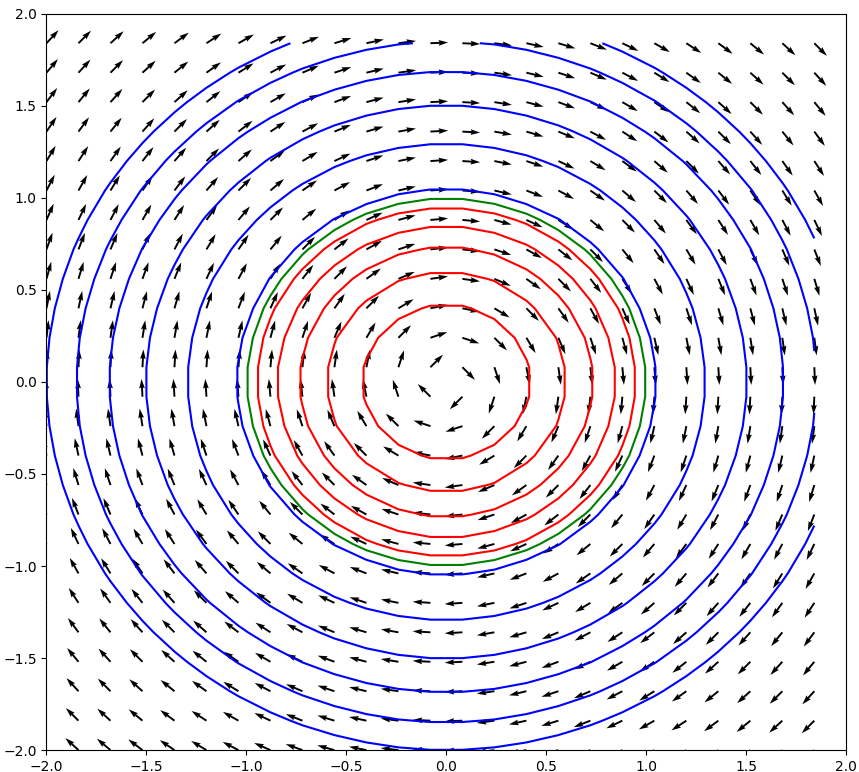
\includegraphics[scale=0.42]{Fig-ex02.png}
\caption{Direction field and implicit solutions of $y' = -\frac{x}{y}$.}
\end{figure}

\begin{figure}[h]
\centering
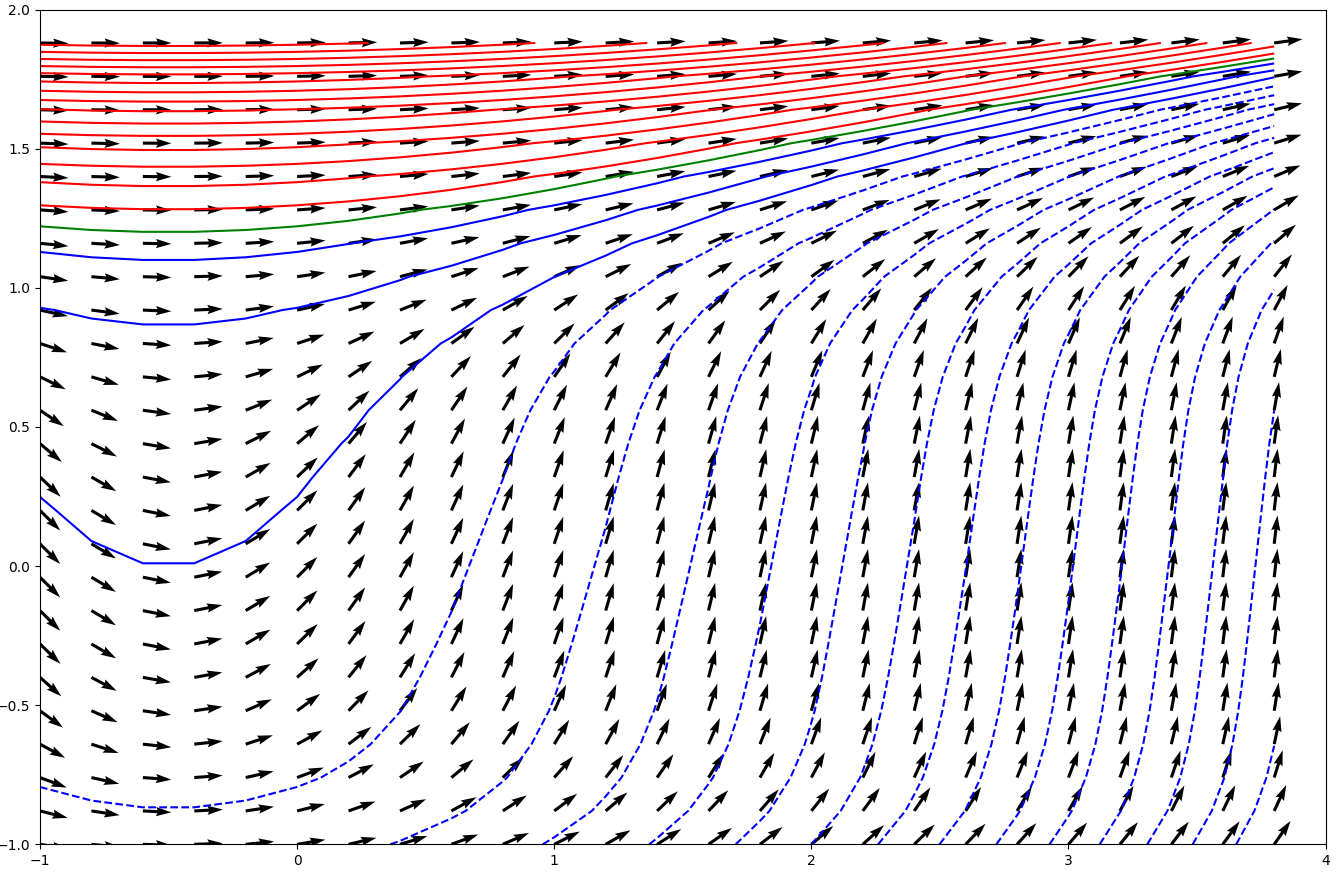
\includegraphics[scale=0.36]{Fig222.png}
\caption{Direction field and implicit solutions of $y' = \frac{2x + 1}{5y^4 + 1}$. In green you can see the implicit solution that satisfies $y(2) = 1$}
\end{figure}

\newpage

\section{Constant Solutions of Separable Equations}
An equation of the form
	\begin{align*}
	y' = g(x) p(y)
	\end{align*}
is separable because it can be put in the following forms:
	\begin{align*}
	\frac{y'}{p(y)} = g(x) .
	\end{align*}

\underline{Problem:}
	\begin{itemize}
	\item The division by $p(y)$ is not possible if $p(y) = 0$.
	\end{itemize}
	
\vspace*{16pt}
	
\begin{example}
Find all solutions to
	\begin{align*}
	y' = 2xy^2 .
	\end{align*}
\end{example}

\newpage

\begin{example}
Find all solutions of
	\begin{align*}
	y' = \frac{1}{2} x (1 - y^2) .
	\end{align*}
\end{example}

\newpage

\phantom{2}

\end{document}